\documentclass[a4paper]{article}

%% Language and font encodings
\usepackage[english]{babel}
\usepackage[utf8x]{inputenc}
\usepackage[T1]{fontenc}

%% Sets page size and margins
\usepackage[a4paper,top=3cm,bottom=2cm,left=3cm,right=3cm,marginparwidth=1.75cm]{geometry}

%% Useful packages
\usepackage{amsmath}
\usepackage{amssymb}
\usepackage{graphicx}
\usepackage{enumerate}
\usepackage[colorinlistoftodos]{todonotes}
\usepackage[colorlinks=true, allcolors=blue]{hyperref}
\usepackage{subfigure}

\title{MTH 9855 Homework 4}
\author{Junliang Zhou}

\begin{document}
\maketitle

\section{Problem 3.1}

If the distribution of $r$ is elliptical, and if $u$ is a standard utility function, then expected utility is a function of mean and variance, and moreover

\[\partial_\mu \hat U(\mu,\omega) \geq 0\]
\[\partial_\omega \hat U(\mu,\omega) \leq 0\]
Show that $d^2\mu/d\sigma^2 >0$, or the rate at which an individual must be compensated for accepting greater $\sigma$ (this rate is $d\mu/d\sigma$) increases as $\sigma$ increases.\newline

\textit{Proof.}\newline

From the lecture we have
\[\mathbb{E}[u(x)]=\int_\mathbb{R} u(\mu+\sigma z) g_1(z^2) dz\]

Take a derivative \textit{w.r.t.} $\sigma$ on both side of the equation,
\[0=\int_\mathbb{R} u'(\mu+\sigma z) \left(\frac{d\mu}{d\sigma}+z\right) g_1(z^2) dz\]

From above we know that
\[\frac{d\mu}{d\sigma}=-\frac{\int_\mathbb{R} u'(\mu+\sigma z) z g_1(z^2) dz}{\int_\mathbb{R} u'(\mu+\sigma z) g_1(z^2) dz}\]

As $u()$ is an increasing concave function and $g_1()$ is a probability density function, we can easily conclude that $d\mu/d\sigma>0$.\newline

Then we take a derivative \textit{w.r.t.} $\sigma$ again on both side of the equation,
\[0=\int_\mathbb{R} \left[ u''(\mu+\sigma z) \left(\frac{d\mu}{d\sigma}+z\right)^2 + u'(\mu+\sigma z) \frac{d^2\mu}{d\sigma^2} \right] g_1(z^2) dz\]

From above we know that
\[\frac{d^2\mu}{d\sigma^2}=-\frac{\int_\mathbb{R} u''(\mu+\sigma z) \left(\frac{d\mu}{d\sigma}+z\right)^2 g_1(z^2) dz}{\int_\mathbb{R} u'(\mu+\sigma z) g_1(z^2) dz}\]

Since we know that $u()$ is a concave function and $\left(\frac{d\mu}{d\sigma}+z\right)^2>0$ for all $z$, it is obvious that $d^2\mu/d\sigma^2 >0$.\newline

\section{Problem 3.2}

Prove that for logarithmic utility, $u(x)=\log x$ and for a log-normal distribution of wealth,

\[f(x;m,s)=\frac{1}{sx\sqrt{2\pi}} \exp{\left(-\frac{(\log x-m)^2}{2s^2}\right)}\]
then the indifference curves are not convex. The moments of $x$ are

\[\mu=e^{m+s^2/2}\]
\[\sigma^2=(e^{m+s^2/2})^2 (e^{s^2}-1)\]
and with a little algebra,

\[\mathbb{E}u=\log \mu-\frac12\log(\sigma^2/\mu^2+1)\]
and then use this to show that for a parametric curve of the form 

\[\mathbb{E}u=\text{constant}\]
$d\mu/d\sigma >0$ everywhere along the curve, but $d^2\mu/d\sigma^2$ changes sign. Verify this on a computer by plotting the relevant curves for various values of the parameters $m$, $s$.\newline

\textit{Proof.}\newline

"$\mathbb{E}u$":\newline

\[\mathbb{E}u=\mathbb{E}\log x=\int_{\mathbb{R}^{+}} \frac{\log x}{sx\sqrt{2\pi}} \exp{\left(-\frac{(\log x-m)^2}{2s^2}\right)} dx\]

Let $y=\log x$, then the integral can be rewrite as

\[\mathbb{E}u=\int_\mathbb{R} \frac{y}{s\sqrt{2\pi}} \exp{\left(-\frac{(y-m)^2}{2s^2}\right)} dy\]

It turns out that $\mathbb{E}u$ is the expectation of a normal distribution with mean $m$ and variance $s^2$, that is
\[\mathbb{E}u=m=\log \mu-\frac12\log(\sigma^2/\mu^2+1)\]

"$\mathbb{E}u=\text{constant}$":\newline

Let $\mathbb{E}u=C_0$ where $C_0$ is a constant in $\mathbb{R}$,
\[\log \mu-\frac12\log(\sigma^2/\mu^2+1)=C_0\]

Take a derivative \textit{w.r.t.} $\sigma$ on both side of the equation,
\[\frac{1}{\mu} \frac{d\mu}{d\sigma}-\frac12 \frac{\mu^2}{\mu^2+\sigma^2} \frac{2\mu^2\sigma-2\mu\sigma^2 \frac{d\mu}{d\sigma}}{\mu^4}=0\]

By simplifying the equation above, we have
\[\frac{d\mu}{d\sigma}=\frac{\mu\sigma}{\mu^2+2\sigma^2}\]

As $\mu$ and $\sigma$ are the mean and variance of a log-normal distributed random variable, they are both positive. Therefore, $d\mu/d\sigma>0$ everywhere.\newline

Take a derivative \textit{w.r.t.} $\sigma$ again,
\[\frac{d^2\mu}{d\sigma^2}=\frac{(\sigma\frac{d\mu}{d\sigma}+\mu)(\mu^2+2\sigma^2)-2(\mu\frac{d\mu}{d\sigma}+2\sigma)\mu\sigma}{(\mu^2+2\sigma^2)^2}\]

Since $\mu$, $\sigma$, and $d\mu/d\sigma$ are all positive, the two terms on the numerator, $(\sigma\frac{d\mu}{d\sigma}+\mu)(\mu^2+2\sigma^2)$ and $-2(\mu\frac{d\mu}{d\sigma}+2\sigma)\mu\sigma$ are positive and negative respectively. As a result, the sign of $d^2\mu/d\sigma^2$ cannot be determined and it's very likely to change as $\mu$ and $\sigma$ vary.\newline

Plot:\newline

The following plots are $\mu$ against $\sigma$ for $m$ varies from 0.25 to 2.\newline

\begin{figure}
\centering
\subfigure[0.25]{\label{fig:a}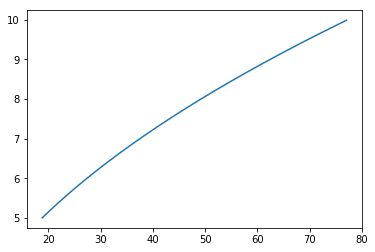
\includegraphics[width=60mm]{2.png}}
\subfigure[0.5]{\label{fig:b}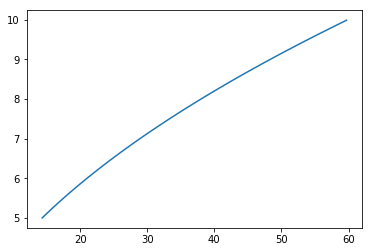
\includegraphics[width=60mm]{3.png}}
\subfigure[0.75]{\label{fig:c}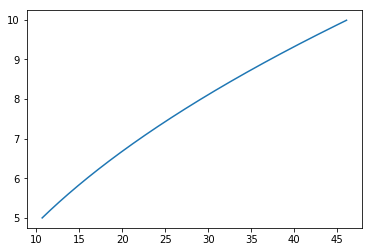
\includegraphics[width=60mm]{4.png}}
\subfigure[1]{\label{fig:d}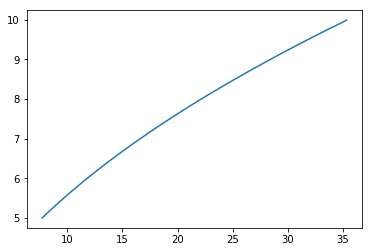
\includegraphics[width=60mm]{5.png}}
\subfigure[1.25]{\label{fig:e}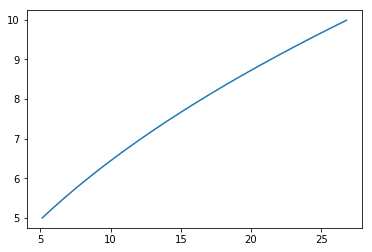
\includegraphics[width=60mm]{6.png}}
\subfigure[1.5]{\label{fig:f}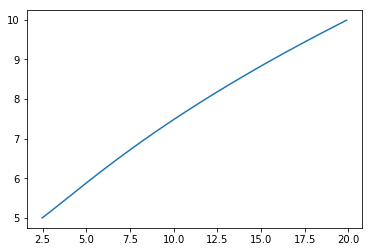
\includegraphics[width=60mm]{7.png}}
\subfigure[1.75]{\label{fig:g}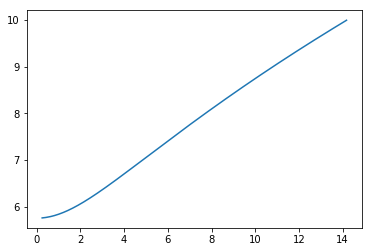
\includegraphics[width=60mm]{8.png}}
\subfigure[2]{\label{fig:h}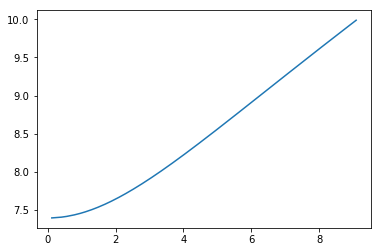
\includegraphics[width=60mm]{9.png}}
\caption{$\mu$ against $\sigma$ plots}
\end{figure}

It is obvious that the convexity changes as $m$ varies.

\end{document}